
\documentclass[a4paper]{article}
\usepackage[margin=2cm]{geometry}

\usepackage[utf8]{inputenc}
% \usepackage[polish]{babel}

\usepackage{color, colortbl}
\usepackage[dvipsnames]{xcolor}
\usepackage{listings}
\usepackage{graphicx}

\usepackage{setspace}

\usepackage{natbib}

\lstset{literate=%
{ą}{{\k{a}}}1
{ć}{{\'c}}1
{ę}{{\k{e}}}1
{ł}{{\l{}}}1
{ń}{{\'n}}1
{ó}{{\'o}}1
{ś}{{\'s}}1
{ż}{{\.z}}1
{ź}{{\'z}}1
{Ą}{{\k{A}}}1
{Ć}{{\'C}}1
{Ę}{{\k{E}}}1
{Ł}{{\L{}}}1
{Ń}{{\'N}}1
{Ó}{{\'O}}1
{Ś}{{\'S}}1
{Ż}{{\.Z}}1
{Ź}{{\'Z}}1,
language=c++,
keywordstyle=\color{gray},
commentstyle=\color{lightgray},
stringstyle=\color{lightgray},
numbers=left,
frame=TBlr,
breaklines=true,
tabsize=2,
numberstyle=\tiny,
basicstyle=\footnotesize \ttfamily
}

\renewcommand\thesection{\arabic{section}.}
\renewcommand\thesubsection{\thesection\arabic{subsection}.}
\renewcommand\thesubsubsection{\thesubsection\arabic{subsubsection}.}
\renewcommand\theparagraph{\thesubsubsection\arabic{paragraph}.}
\renewcommand\thesubparagraph{\theparagraph\arabic{subparagraph}.}

\title{Softcomputing \\ Translation system based on a Multilayer Perceptron: pictures of characters and digits into a Braille alphabet
signs - Report}
\author{\textbf{Krystian Horecki} 181079 \\ 
	\textbf{Antoni Buszta} 181013 \\
	Wroclaw University of Technology}
\date{15.11.2013 r.}

\begin{document}

\maketitle
\newpage
\onehalfspace

\section{Project description}
\subsection{Project goals} 
The goal of the project was to create automatic translation mechanism from pictures of characters to Brail alphabet signs.
Pictures of the characters were supposed to be a source of input and training data for translation mechanism.
Translation engine was supposed to be created in form of Multilayer Perceptron which is kind of artificial neural network.
Important challenge was to create engine which allows to recognize and translate as many characters as it's possible and with many different distortions of different levels.
There was no requirement to create user interface in order to focus on engine properties and results instead of good project appearance.
\subsection{Input data format}
Characters which were used as a source of input data were presented in form of images which were converted to tables containing boolean values.
This conversion allowed us to make input data more friendly for further processing. At the same time data still contained exactly the same data as picture and could be converted to this form in any time.
Example table containing character of capital \textbf{A} was presented below. \\
\begin{center}
		[0, 0, 0, 0, 0, 0, 0, 0, 0, 0,\\
        0, 0, 0, 0, 0, 0, 0, 0, 1, 0,\\
        0, 0, 1, 1, 1, 1, 1, 1, 1, 0,\\
        0, 1, 0, 0, 0, 1, 0, 0, 1, 0,\\
        1, 0, 0, 0, 0, 1, 0, 0, 0, 0,\\
        1, 0, 0, 0, 0, 1, 0, 0, 0, 0,\\
        0, 1, 0, 0, 0, 1, 0, 0, 1, 0,\\
        0, 0, 1, 1, 1, 1, 1, 1, 1, 0,\\
        0, 0, 0, 0, 0, 0, 0, 0, 1, 0,\\
        0, 0, 0, 0, 0, 0, 0, 0, 0, 0]\\
\end{center}
 
\subsection{Translation mechanism}
As a translation mechanism Multilayer Perceptron was used. To create MP we used Python programming language and pyBrain library which allows to easily create neural network with required nodes configuration.
Preparing project we were experimenting with following properties of network:
\begin{itemize}
	\item number of hidden layers
	\item number of neurons in hidden layer
	\item types of hidden layer
	\item types of output layer
	\item output data presentation methods
\end{itemize}
Results of those experiments were presented later in this paper.

\subsection{Output data format}
During experiments we decided to check 2 different approaches of output data computing:
\begin{enumerate}
	\item \textbf{Translation:} Encoded Brail alphabet characters in form of table, one output neuron refers to one position in table 
	\item \textbf{Clasification:} One output neuron per one class, which means that each output neuron represents different Brail symbol
\end{enumerate}
Because those two methods mean that different number of output neurons are used they can give different translation results.
Results of testing those two approaches were presented later in this paper.

\section{Used preprocessing and post processing methods}
\subsection{Preprocessing} 
To make network more sensitive to black and white pixels which are presented in input data as 0 and 1 we made function converting all zeros to -1.
It allowed to improve learning and testing results irrespective of output data computation method(classification or direct translation).
\subsection{Post processing}
In case of post processing, used method depended on output data computation method, which means that two different post processing methods were used:
\subsubsection{Translation post processing method}
Post processing was based on assumption that neural network output was in form float numbers table.
To create final result we rounded those numbers to 1 or 0 which gave us proper result.
\subsubsection{Classification post processing method}
During classification neural network as a result gives us table of float numbers with values referring to different classes of output data.
To decide which class is a proper one we used method choosing the biggest value from the table. The index of the biggest value was used to determine final class of object recognized by neural network. 

\section{Training sets and methods}
As a training set the pool of capital letters was used. Each letter was represented in set 300 times to make it easier to learn network. During preparations few tests for optimal learning were done with following properties as a variable:
\begin{itemize}
	\item Learning epochs number
	\item Number of hidden neurons
	\item Learning rate
	\item Momentum - value for parameters of network are adjusted
\end{itemize}

On figure \ref{epochs} it can be seen how average number of maximum noisy pixels changes along with number of training epoch. Network behavior was tested with both translation and classification methods, which also can be seen on chart.
\begin{figure}[ht]
	\centering
	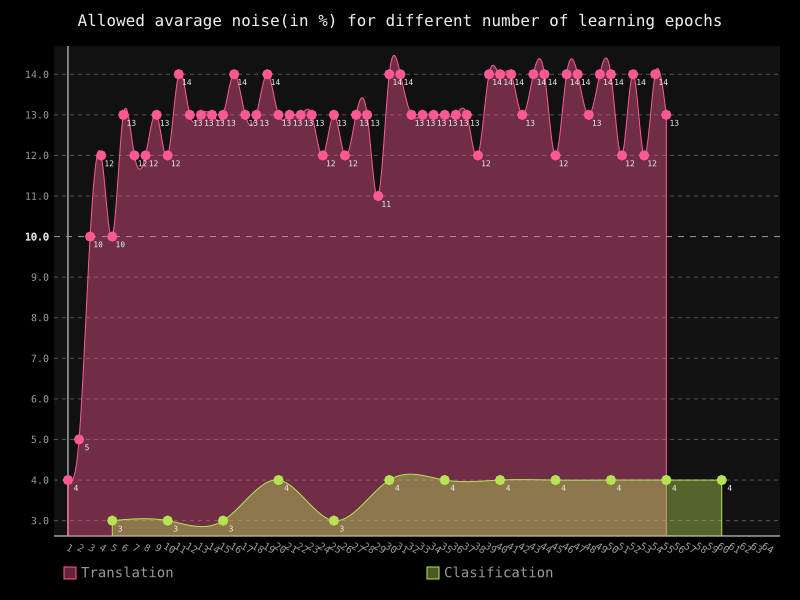
\includegraphics[scale=0.7,keepaspectratio=true]{Charts/epochsChart.png}	
	\caption{}
	\label{epochs}
\end{figure}
After tests we decided to use 55 training epochs to provide sufficient training level for network.
It was also tested how number of hidden neurons affects results of characters recognition.
As it can be seen on figure \ref{hidden} that relatively good results we get with 55 hidden neurons so this number was later used for tests.
\begin{figure}[ht]
	\centering
	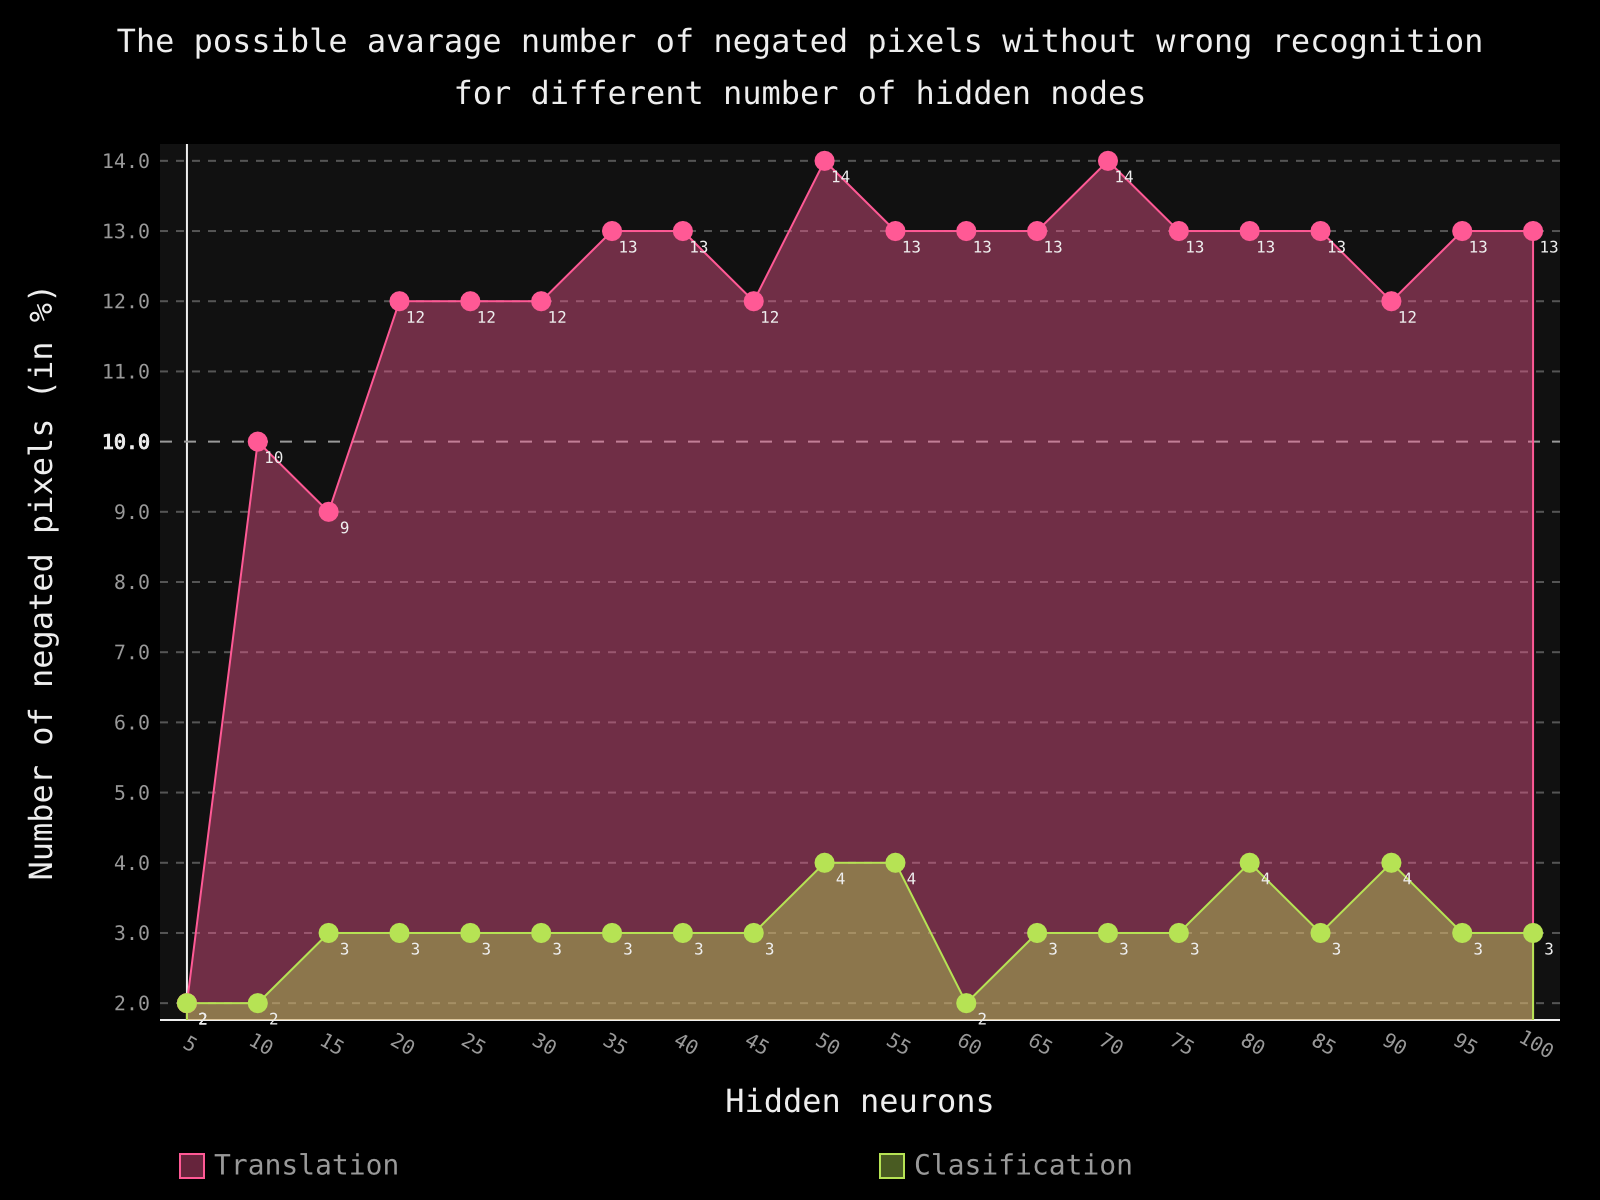
\includegraphics[scale=0.7,keepaspectratio=true]{Charts/hiddenChart.png}	
	\caption{}
	\label{hidden}
\end{figure} 

On figure \ref{learn} we can see that learning rate has no significant influence on later results, learning rate with value 0.016 was used for later tests.
\begin{figure}[ht]
	\centering
	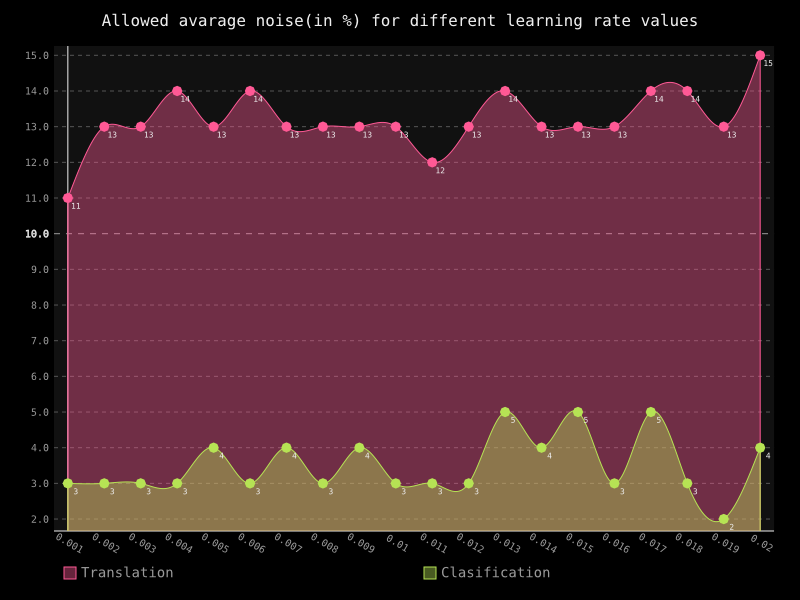
\includegraphics[scale=0.7,keepaspectratio=true]{Charts/learnChart.png}	
	\caption{}
	\label{learn}
\end{figure} 

Analysing chart on figure \ref{momentum} it can be seen that best value of momentum is oscillating around 0.95 and that value was chosen for later tests.
\begin{figure}[ht]
	\centering
	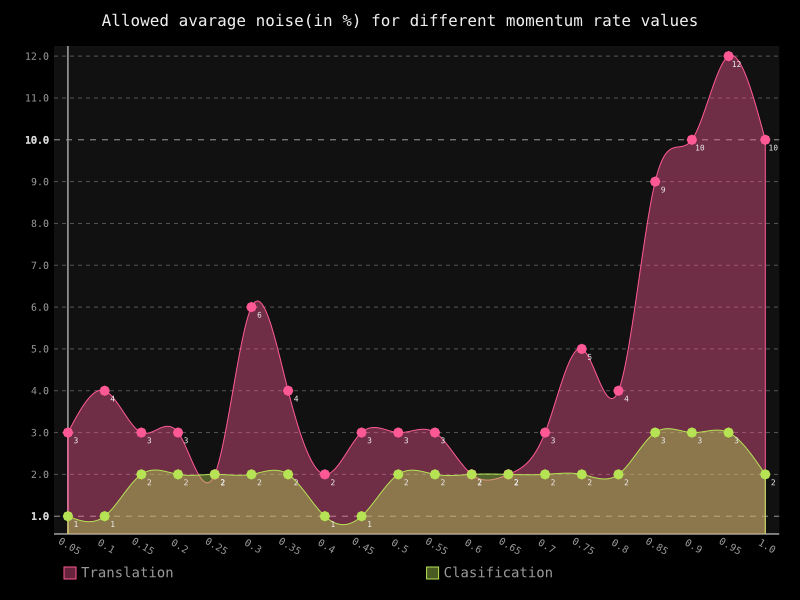
\includegraphics[scale=0.7,keepaspectratio=true]{Charts/momentumChart.png}	
	\caption{}
	\label{momentum}
\end{figure}

\clearpage
Final training was done with following parameters:
\begin{itemize}
	\item Training epochs: 55
	\item Number of hidden neurons: 55
	\item Learning rate: 0.016
	\item Momentum: 0.95
\end{itemize}
\clearpage
\pagebreak
\section{Engine description}

After training and tests we decided to create Multilayer Perceptron with 1 hidden layer and 55 hidden neurons. During experiments it occurred that the best results in case of classification we get using Softmax hidden and output layer type. For translation the best was Sigmoid layer type so it was used.

\section{Gained results}
\subsection{Test description}
Below are presented all gained tests results for prepared tests with short description.
We have tested our engine for both:
\begin{itemize}
  \item Translation
  \item Classification
\end{itemize}
Engine was tested with following type of tests:
\begin{itemize}
	\item Number of random pixels negation
	\item One vertical line removal success rate 
	\item One horizontal line removal success rate
	\item Number of random vertical lines removal
	\item Number of random horizontal lines removal
	\item Square with random position and particular size removal
	\item Number of adjacent to character pixels
\end{itemize}
More accurate description was presented in subsection which concerns each test type.

\clearpage
\subsection{Number of random pixels negation}
Test was performed for increasing number of random pixels which were negated. Number of negated pixels was increased as long as wrong recognition occured. This was repeated 100 times and avarage number of negated pixels for wrong recognition was returned for each letter as a result. Figures \ref{noise_trans} and \ref{noise_clas} show results of tests for clasification and translation. 
\begin{figure}[ht]
	\centering
	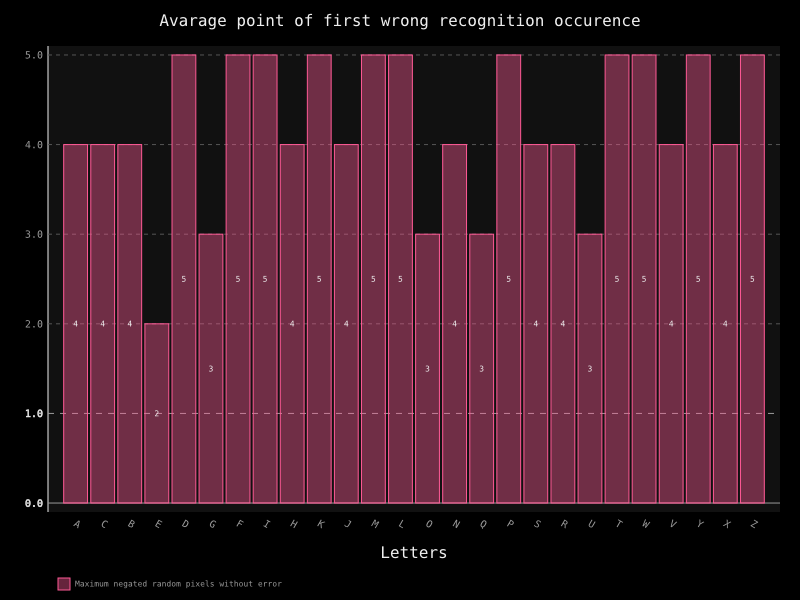
\includegraphics[scale=0.7,keepaspectratio=true]{Charts/RandNoiseTestPlanResultsChart_NormalTester.png}	
	\caption{}
	\label{noise_trans}
\end{figure}

\begin{figure}[t]
	\centering
	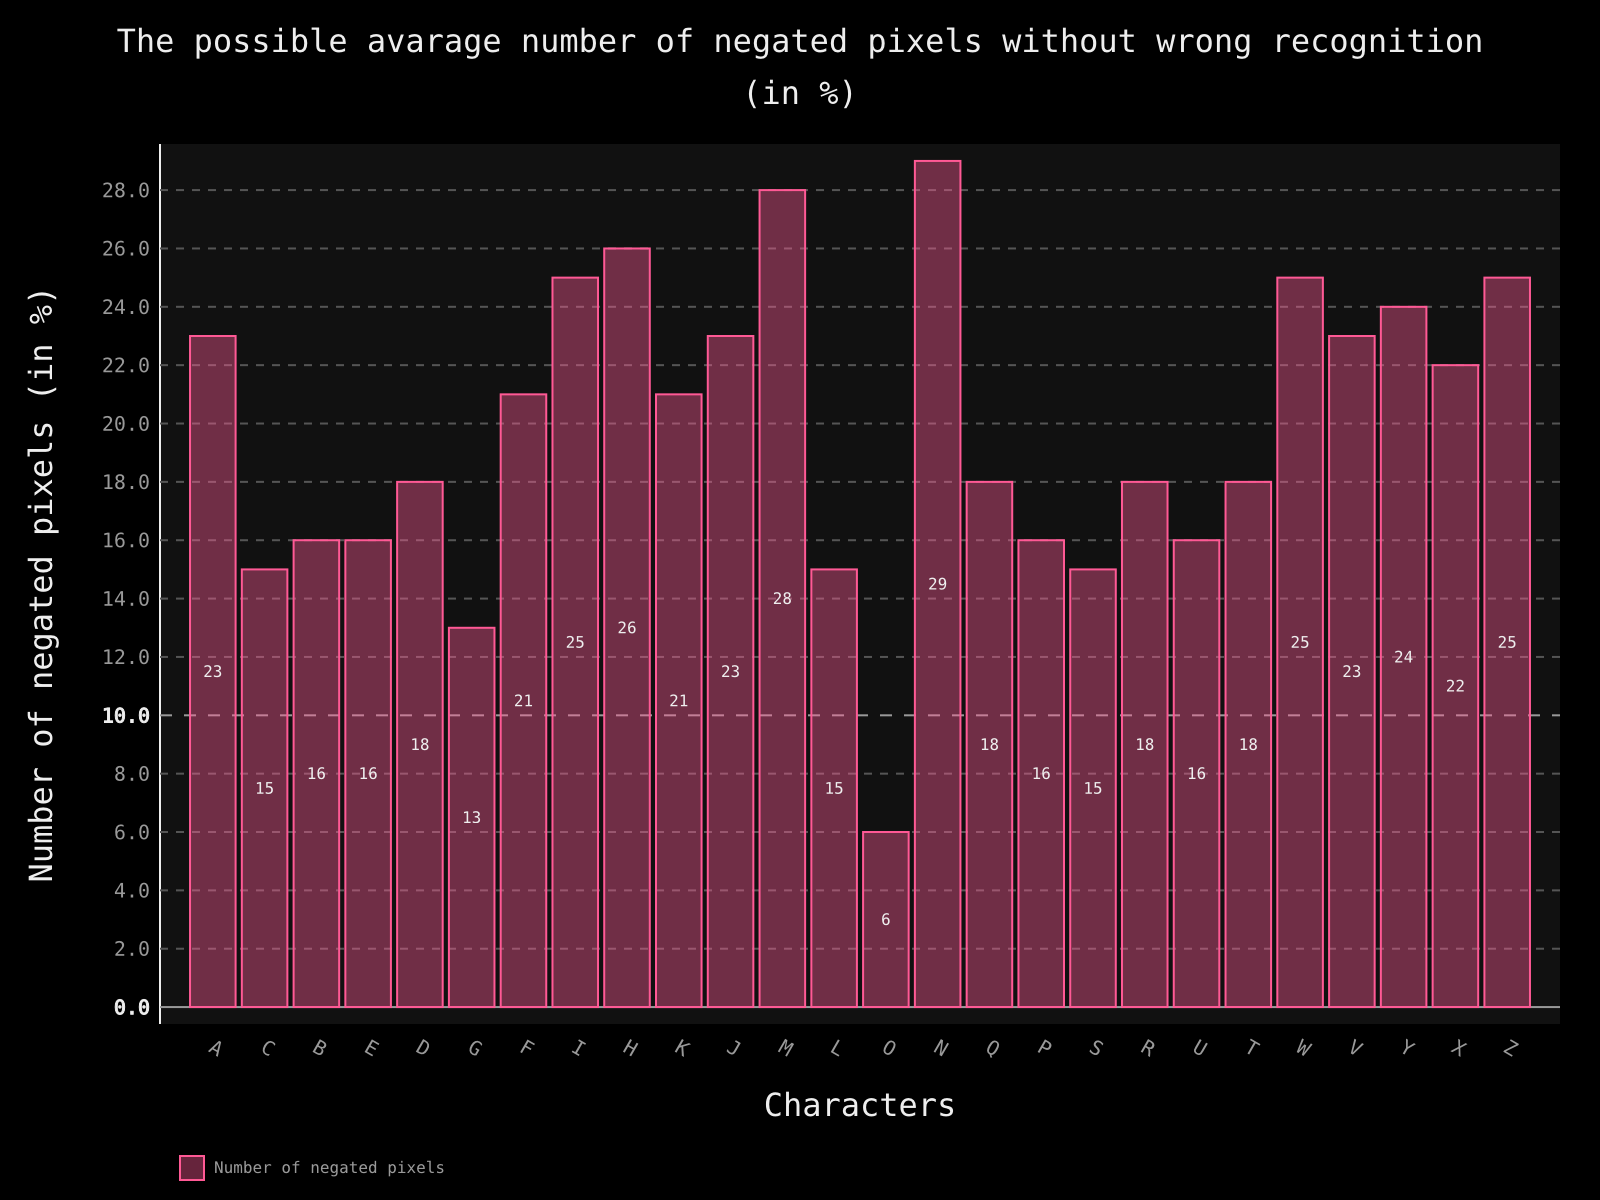
\includegraphics[scale=0.7,keepaspectratio=true]{Charts/RandNoiseTestPlanResultsChart_ClasifierTester.png}	
	\caption{}
	\label{noise_clas}
\end{figure}

\clearpage
\subsection{One vertical line removal success rate}
In test each one vertical line of character was removed. As a result test returned succes rate of this removal, which for both methods was presented on figures \ref{ver_line_trans} and \ref{ver_line_clas}.
\begin{figure}[ht]
	\centering
	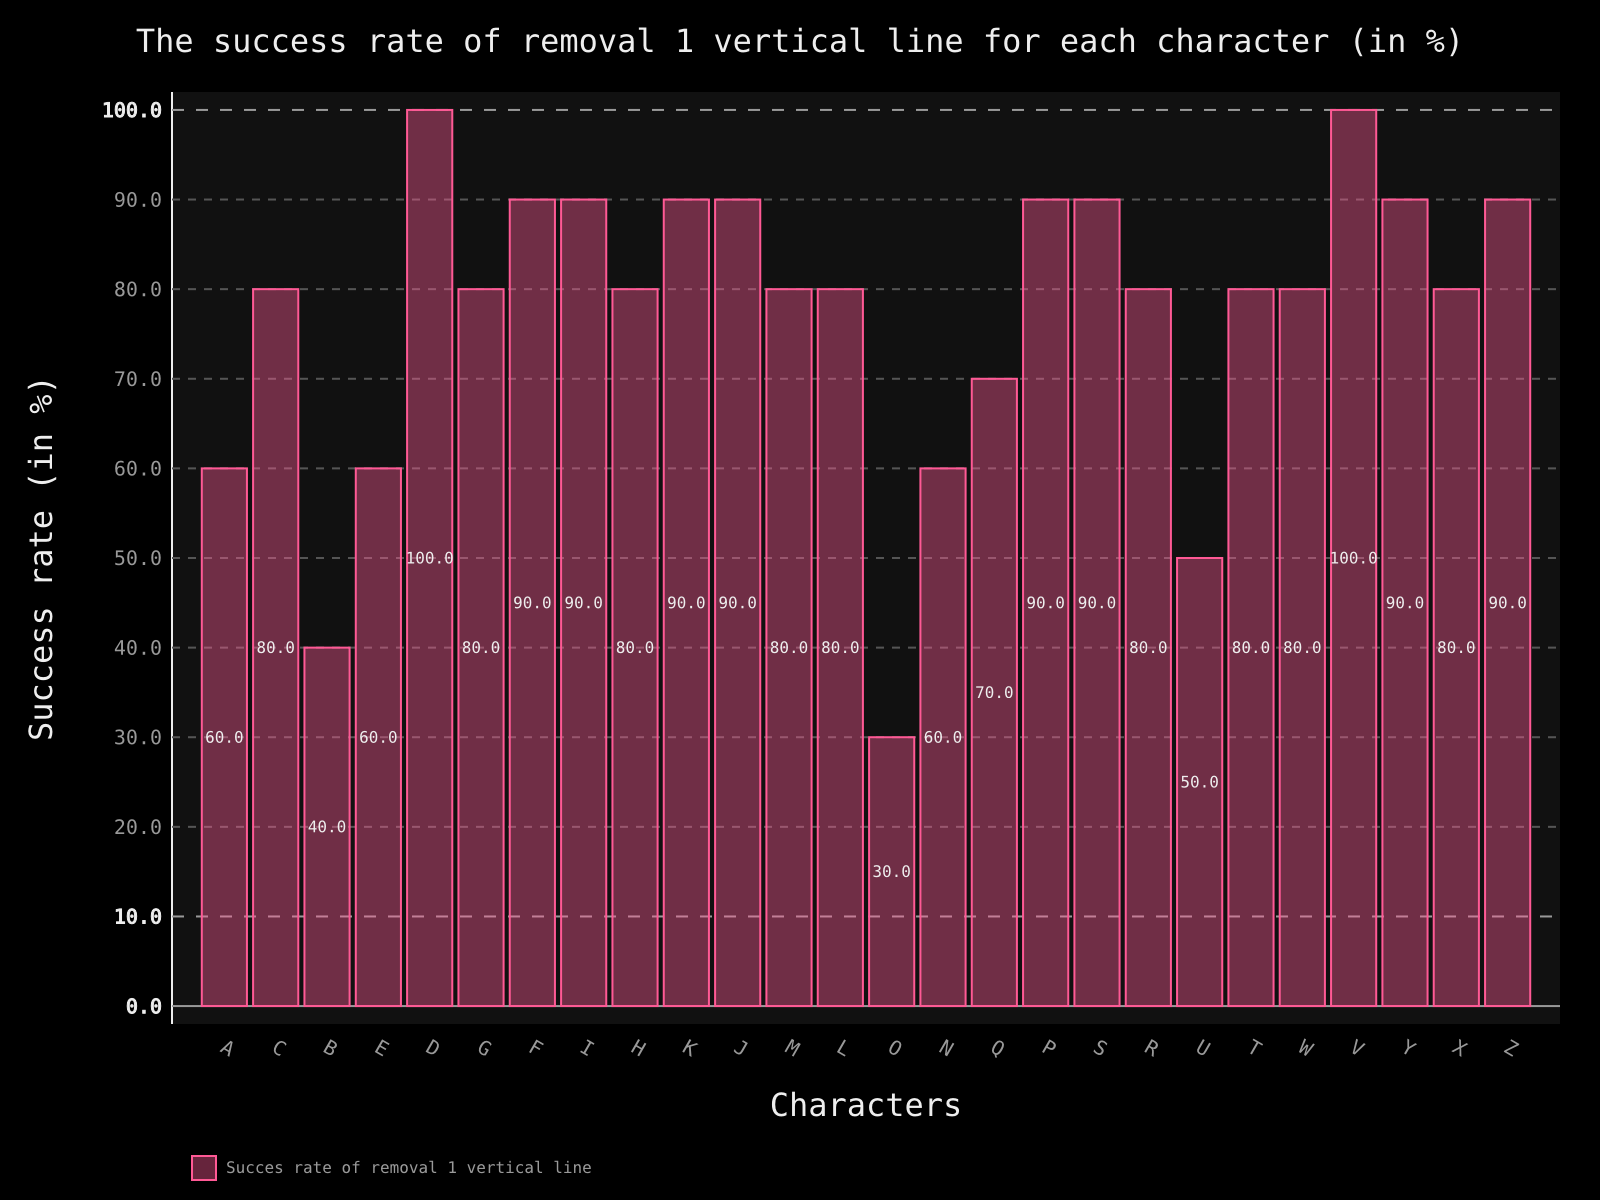
\includegraphics[scale=0.7,keepaspectratio=true]{Charts/VerLineTestPlanResultsChart_NormalTester.png}	
	\caption{}
	\label{ver_line_trans}
\end{figure}

\begin{figure}[t]
	\centering
	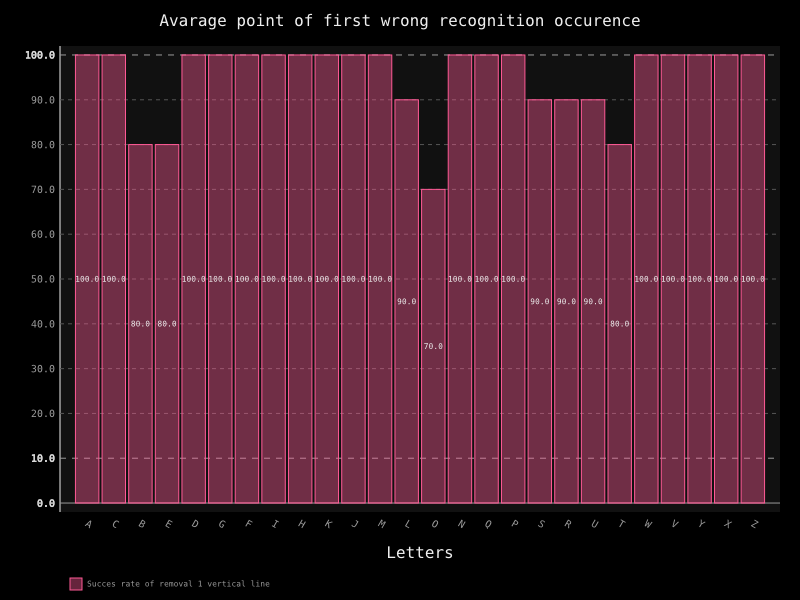
\includegraphics[scale=0.7,keepaspectratio=true]{Charts/VerLineTestPlanResultsChart_ClasifierTester.png}	
	\caption{}
	\label{ver_line_clas}
\end{figure}


\clearpage
\subsection{One horizontal line removal success rate}
In test each one horizontal line of character was removed. As a result test returned succes rate of this removal, which for both methods was presented on figures \ref{hor_line_trans} and \ref{hor_line_clas}.
\begin{figure}[ht]
	\centering
	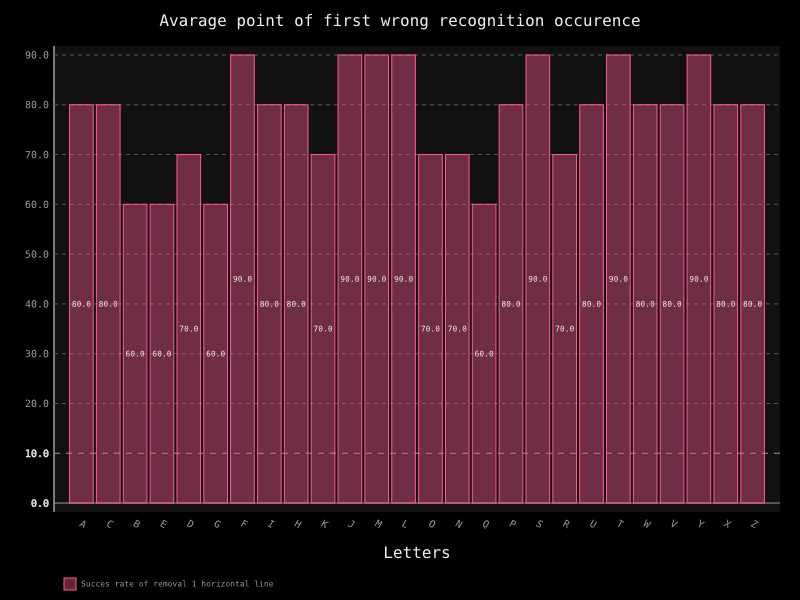
\includegraphics[scale=0.7,keepaspectratio=true]{Charts/HorLineTestPlanResultsChart_NormalTester.png}	
	\caption{}
	\label{hor_line_trans}
\end{figure}

\begin{figure}[t]
	\centering
	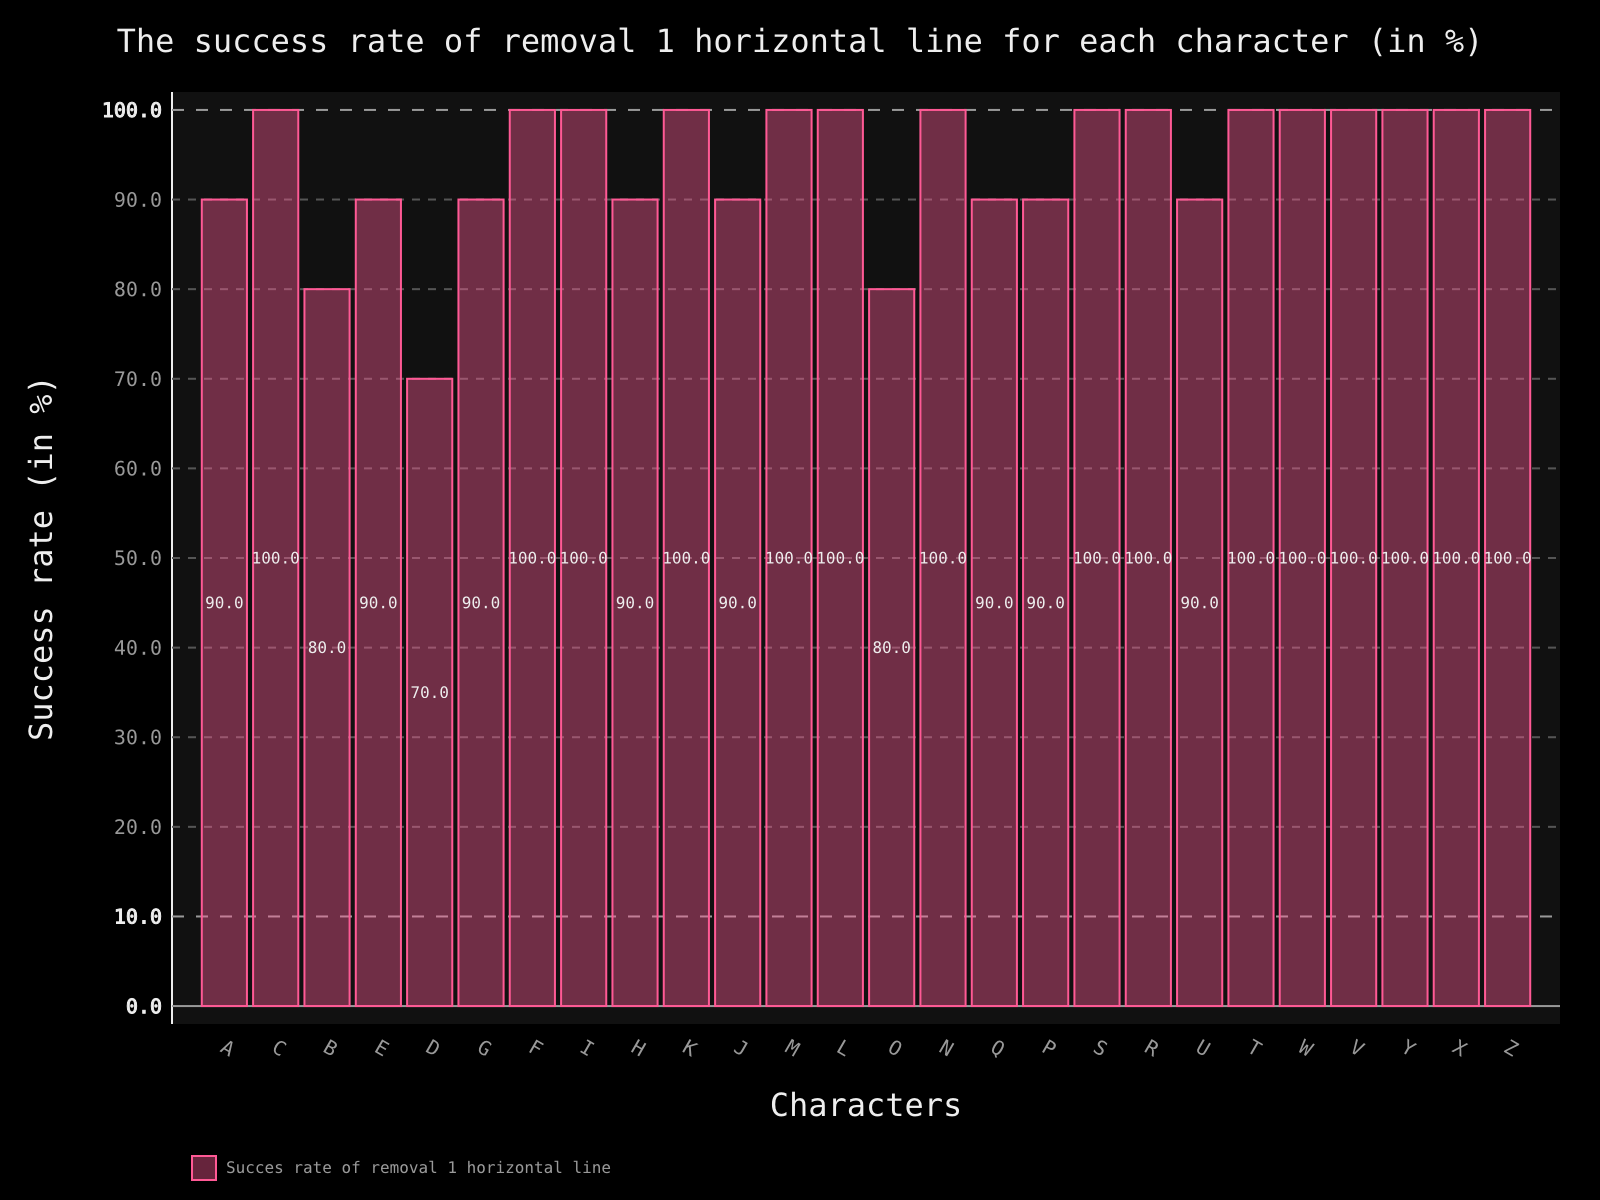
\includegraphics[scale=0.7,keepaspectratio=true]{Charts/HorLineTestPlanResultsChart_ClasifierTester.png}	
	\caption{}
	\label{hor_line_clas}
\end{figure}

\clearpage
\subsection{Number of random vertical lines removal}
Test was performed for increasing number of random vertical lines which were removed. Number of vertical lines was increased as long as wrong recognition occured. This was repeated 100 times and avarage number of vertical lines for wrong recognition was returned for each letter as a result. Figures \ref{ver_lines_trans} and \ref{ver_lines_clas} show results of tests for clasification and translation. 
\begin{figure}[ht]
	\centering
	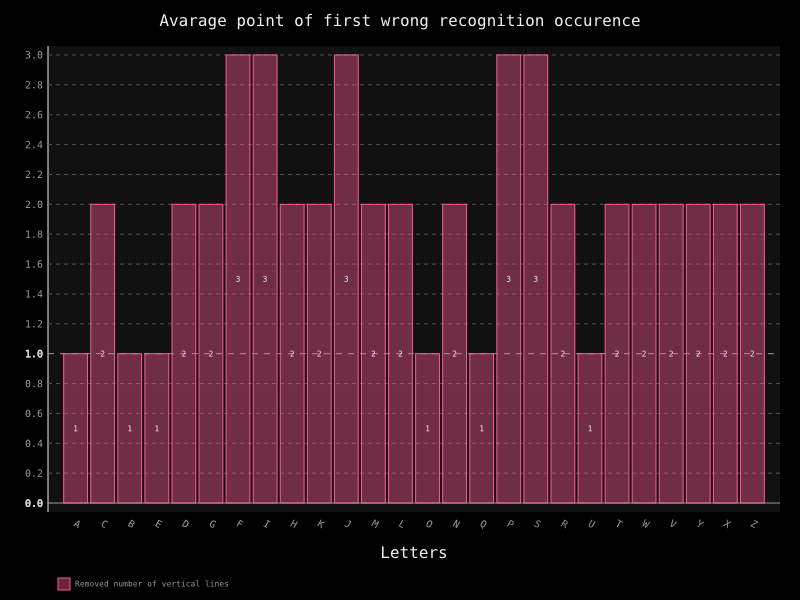
\includegraphics[scale=0.7,keepaspectratio=true]{Charts/LinesVerTestPlanResultsChart_NormalTester.png}	
	\caption{}
	\label{ver_lines_trans}
\end{figure}

\begin{figure}[t]
	\centering
	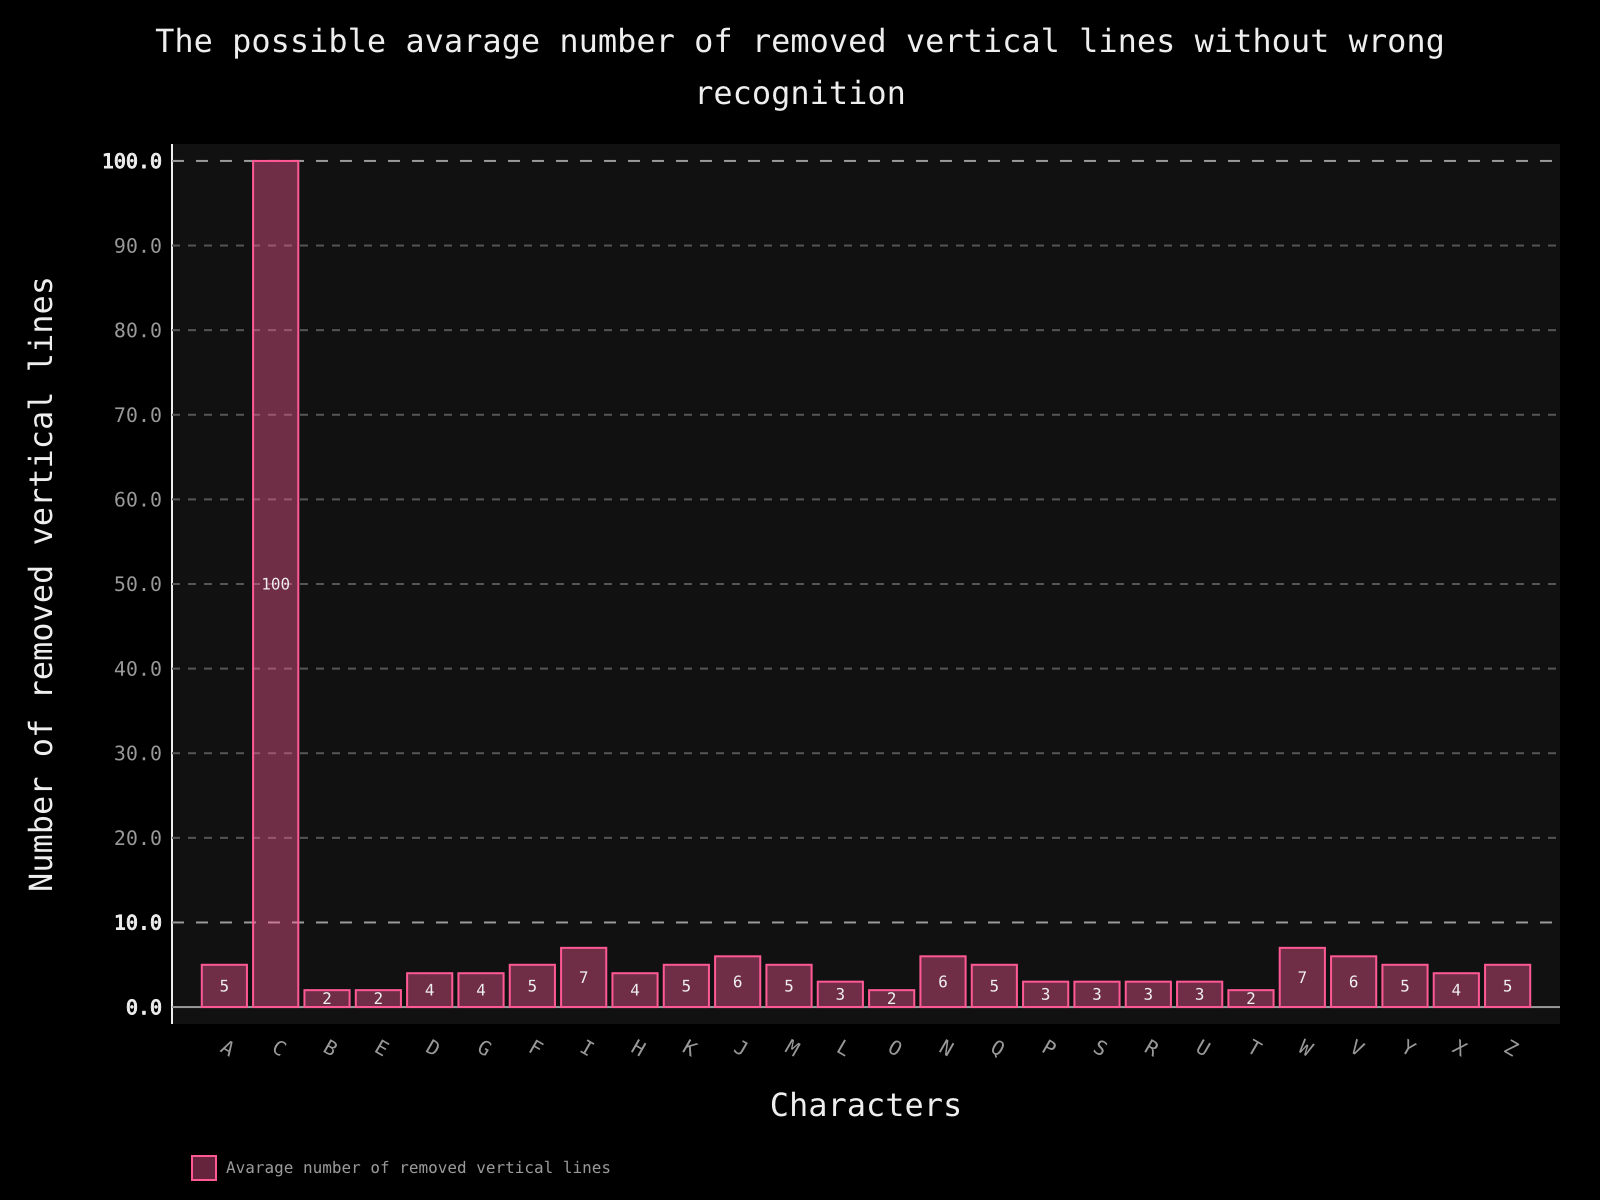
\includegraphics[scale=0.7,keepaspectratio=true]{Charts/LinesVerTestPlanResultsChart_ClasifierTester.png}	
	\caption{}
	\label{ver_lines_clas}
\end{figure}


\clearpage
\subsection{Number of random horizontal lines removal}
Test was performed for increasing number of random horizontal lines which were removed. Number of horizontal lines was increased as long as wrong recognition occured. This was repeated 100 times and avarage number of horizontal lines for wrong recognition was returned for each letter as a result. Figures \ref{hor_lines_trans} and \ref{hor_lines_clas} show results of tests for clasification and translation. 
\begin{figure}[ht]
	\centering
	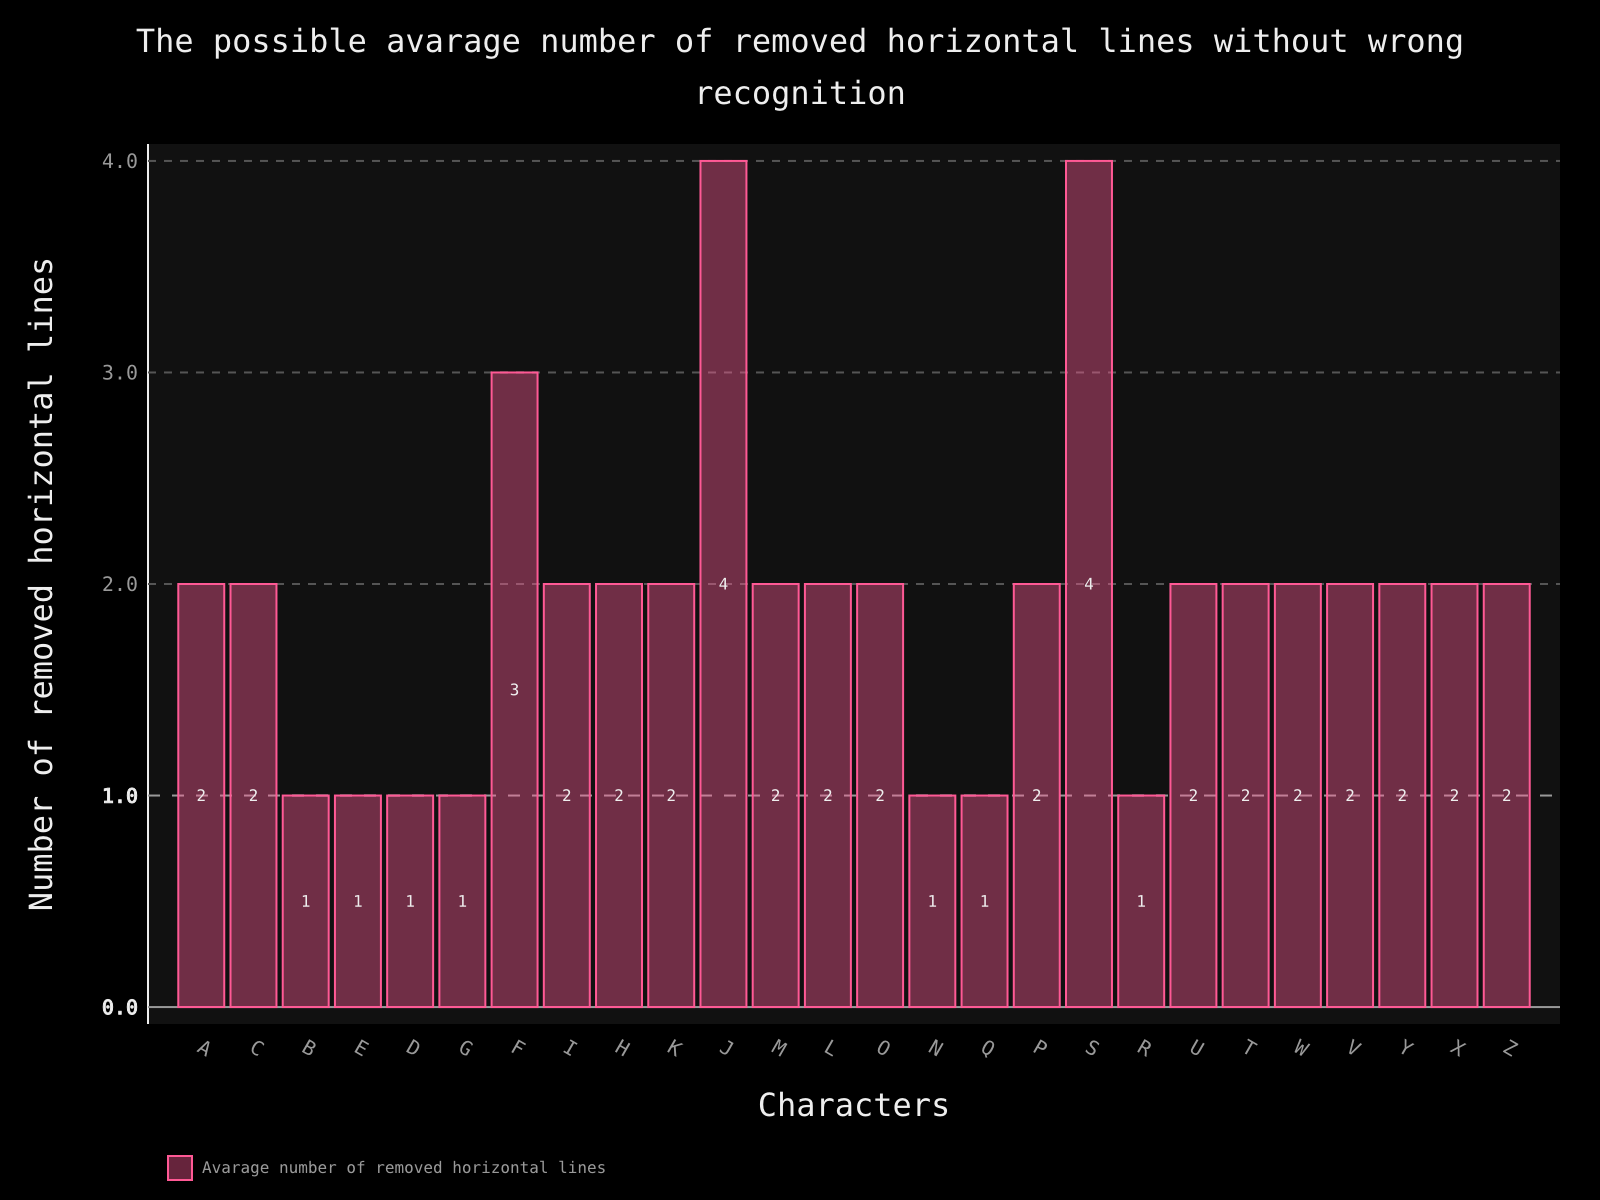
\includegraphics[scale=0.7,keepaspectratio=true]{Charts/LinesHorTestPlanResultsChart_NormalTester.png}	
	\caption{}
	\label{hor_lines_trans}
\end{figure}

\begin{figure}[t]
	\centering
	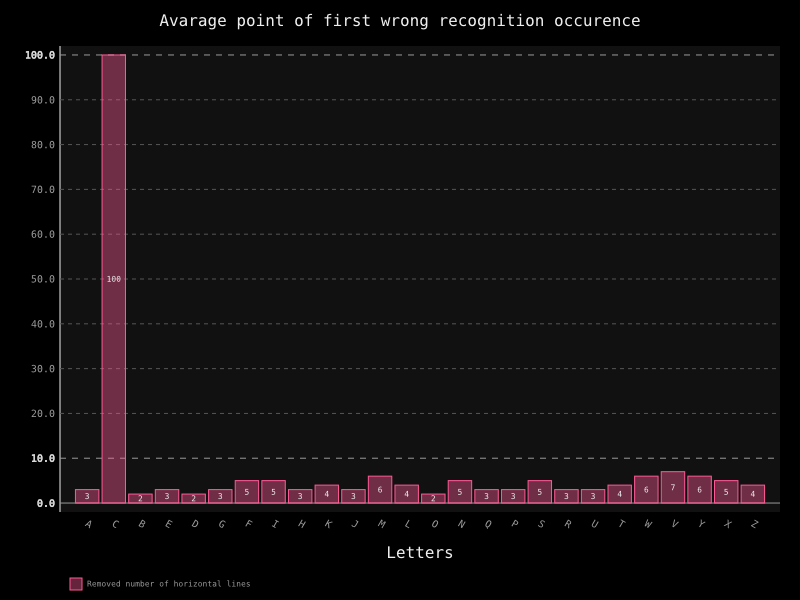
\includegraphics[scale=0.7,keepaspectratio=true]{Charts/LinesHorTestPlanResultsChart_ClasifierTester.png}	
	\caption{}
	\label{hor_lines_clas}
\end{figure}


\clearpage
\subsection{Number of random horizontal and vertical lines removal comprasion}
Test for removal of number of random vertical and horizontal lines were accumulated in one chart.
Figures \ref{lines_trans} and \ref{lines_clas} show results of tests for clasification and translation. 
\begin{figure}[ht]
	\centering
	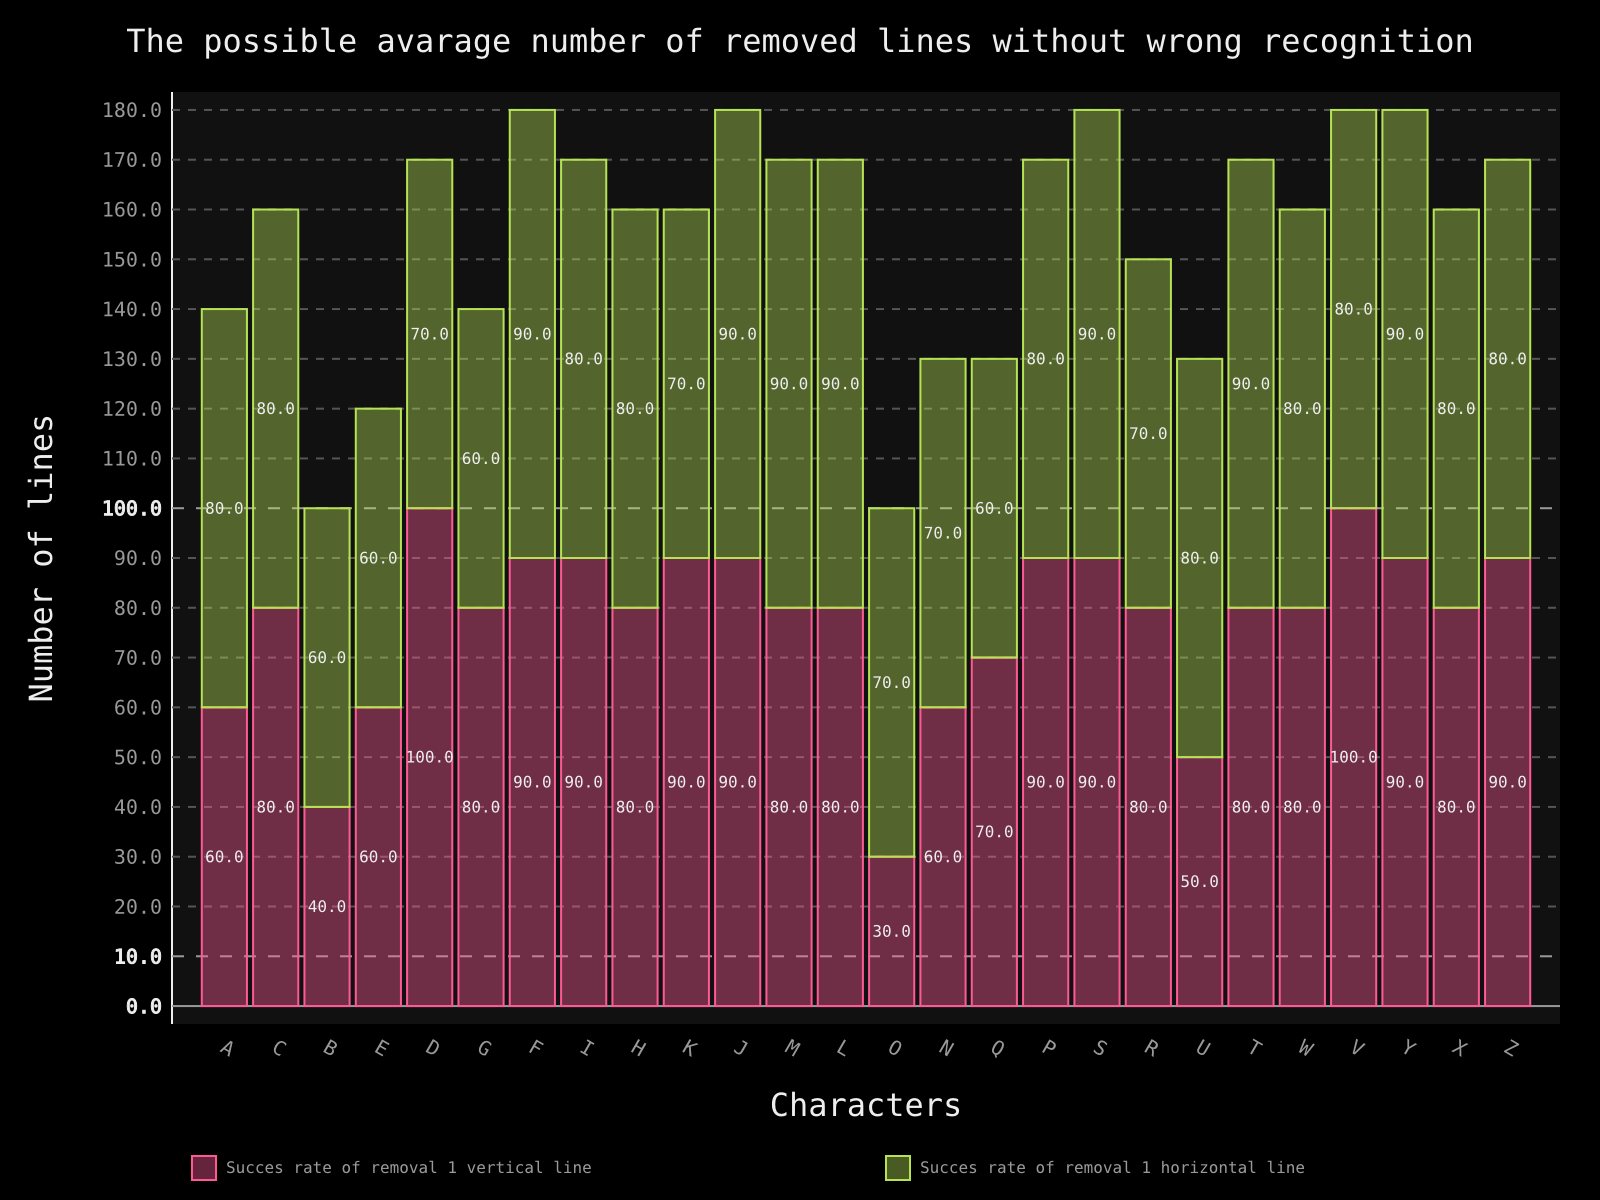
\includegraphics[scale=0.7,keepaspectratio=true]{Charts/Removed_linesTestPlanResultsChart_NormalTester.png}	
	\caption{}
	\label{lines_trans}
\end{figure}

\begin{figure}[t]
	\centering
	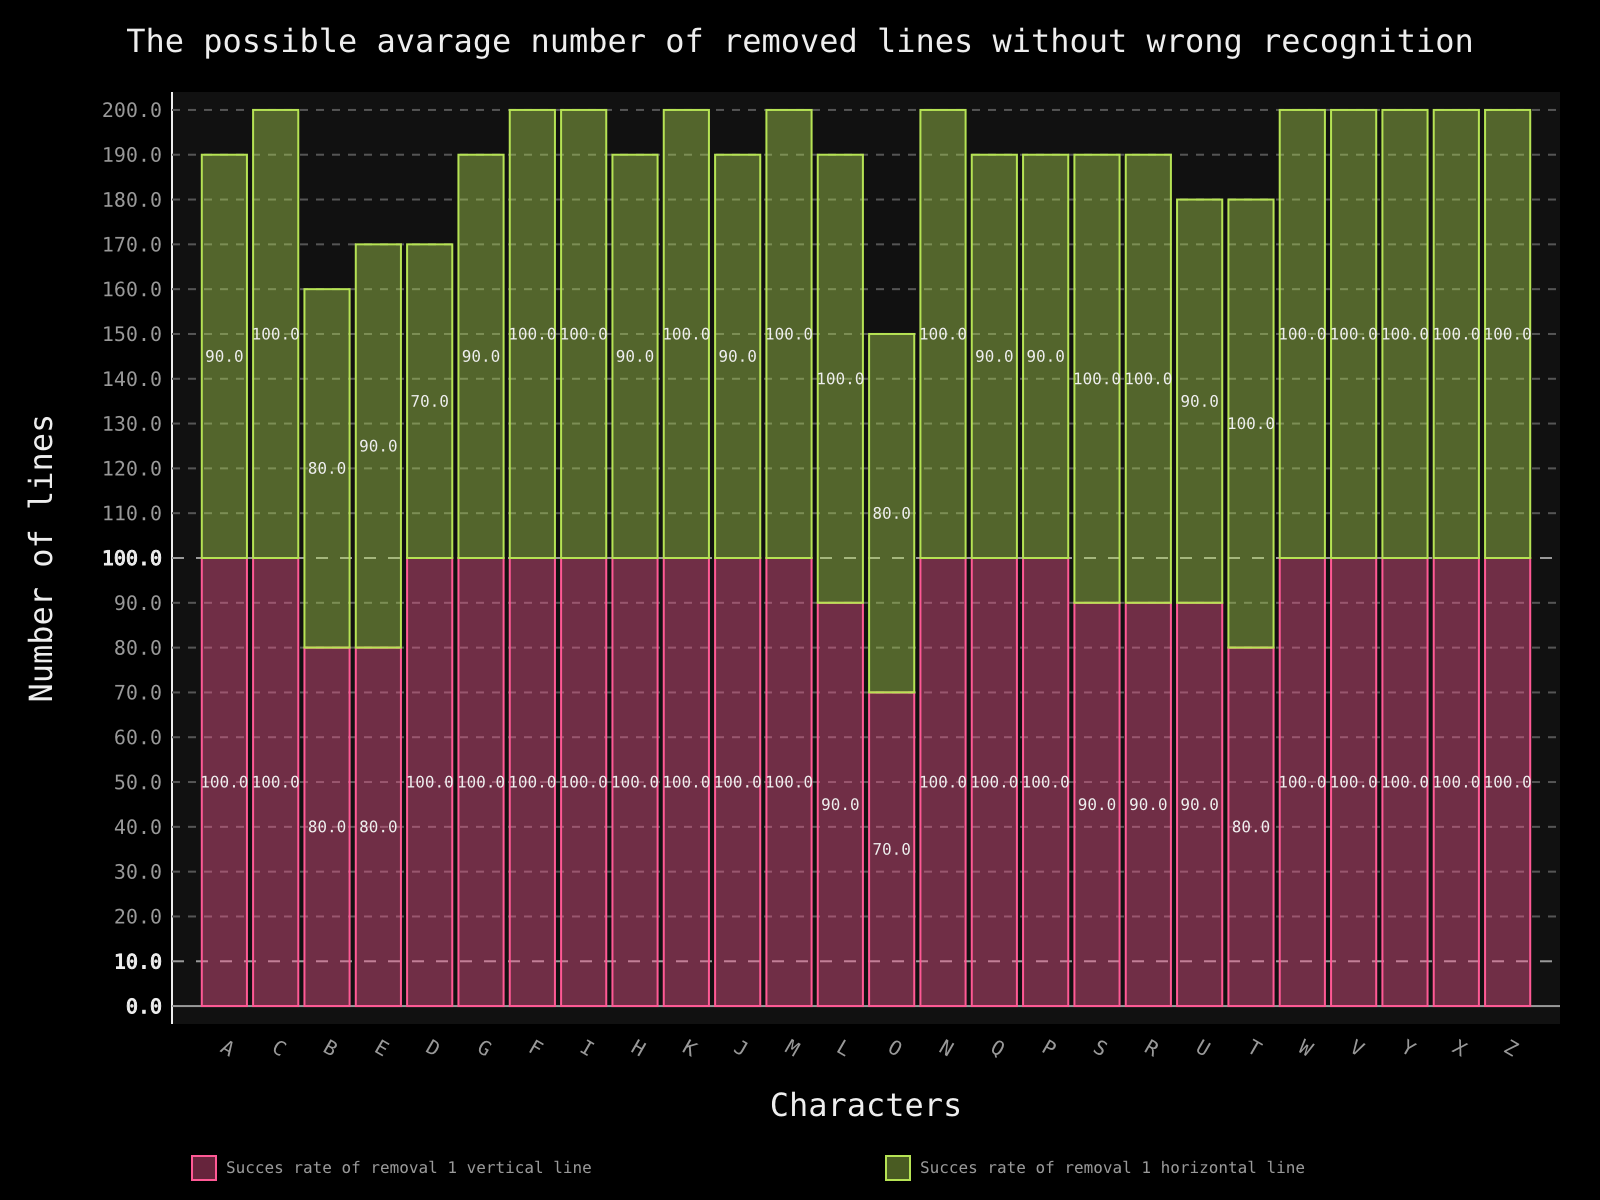
\includegraphics[scale=0.7,keepaspectratio=true]{Charts/Removed_linesTestPlanResultsChart_ClasifierTester.png}	
	\caption{}
	\label{lines_clas}
\end{figure}

\clearpage
\subsection{Square with random position and particular size removal}
Test was performed for increasing size of randomly located square which was removed from character picture. Size of square was increased as long as wrong recognition occured. This was repeated 100 times and avarage size of square for wrong recognition was returned for each letter as a result. Figures \ref{squares_trans} and \ref{squares_clas} show results of tests for clasification and translation. 
\begin{figure}[ht]
	\centering
	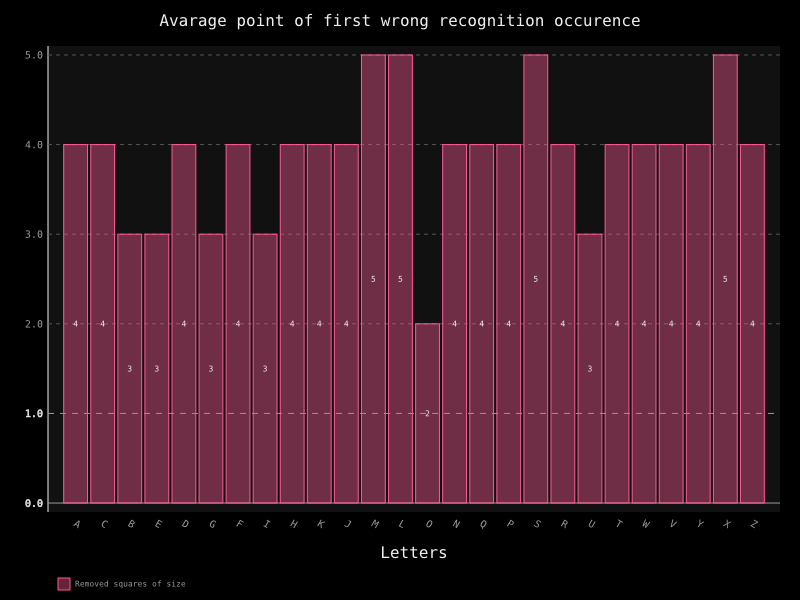
\includegraphics[scale=0.7,keepaspectratio=true]{Charts/SquaresTestPlanResultsChart_NormalTester.png}	
	\caption{}
	\label{squares_trans}
\end{figure}

\begin{figure}[t]
	\centering
	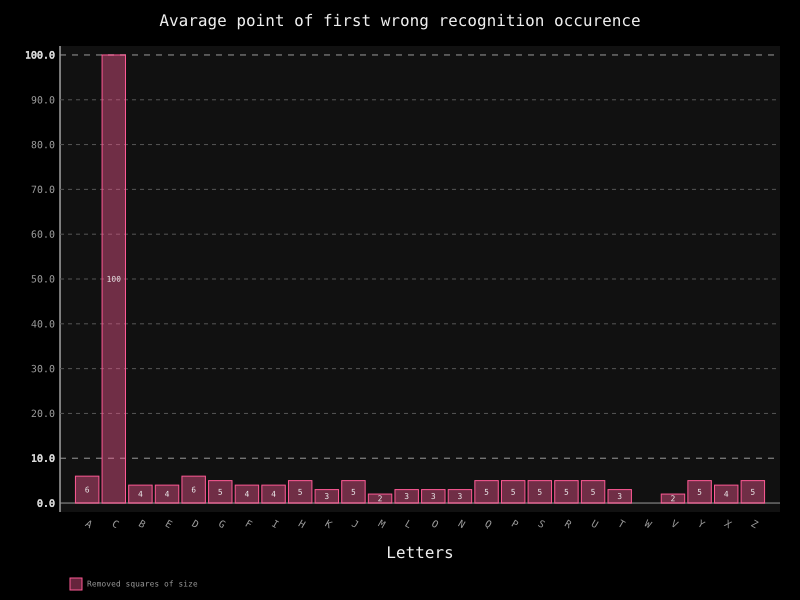
\includegraphics[scale=0.7,keepaspectratio=true]{Charts/SquaresTestPlanResultsChart_ClasifierTester.png}	
	\caption{}
	\label{squares_clas}
\end{figure}


\clearpage
\subsection{Number of adjacent to character pixels}
Test was performed for increasing number of randomly located adjacent pixels which were coloured on characters picture. Number of pixels was increased as long as wrong recognition occured. This was repeated 100 times and avarage number of adjacent pixels for wrong recognition was returned for each letter as a result. Figures \ref{adjacent_trans} and \ref{adjacent_clas} show results of tests for clasification and translation.
\begin{figure}[ht]
	\centering
	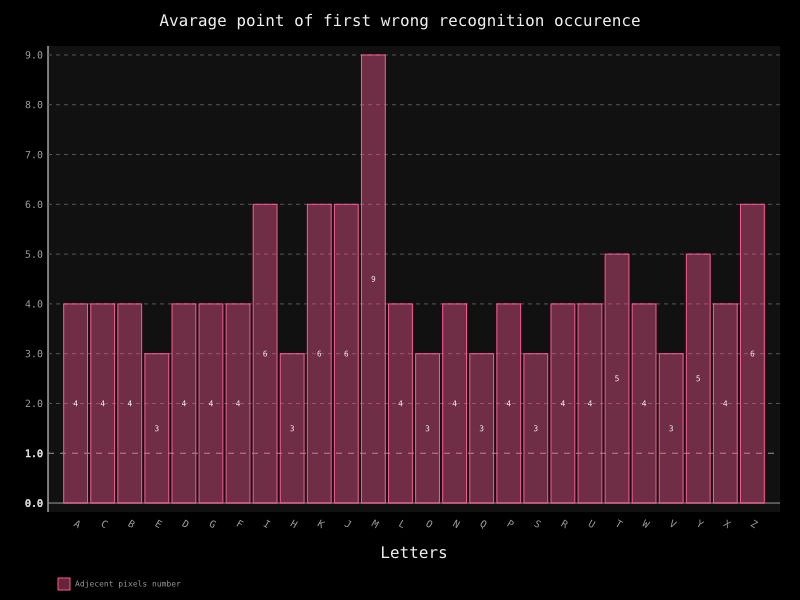
\includegraphics[scale=0.7,keepaspectratio=true]{Charts/AdjecentTestPlanResultsChart_NormalTester.png}	
	\caption{}
	\label{adjacent_trans}
\end{figure}

\begin{figure}[t]
	\centering
	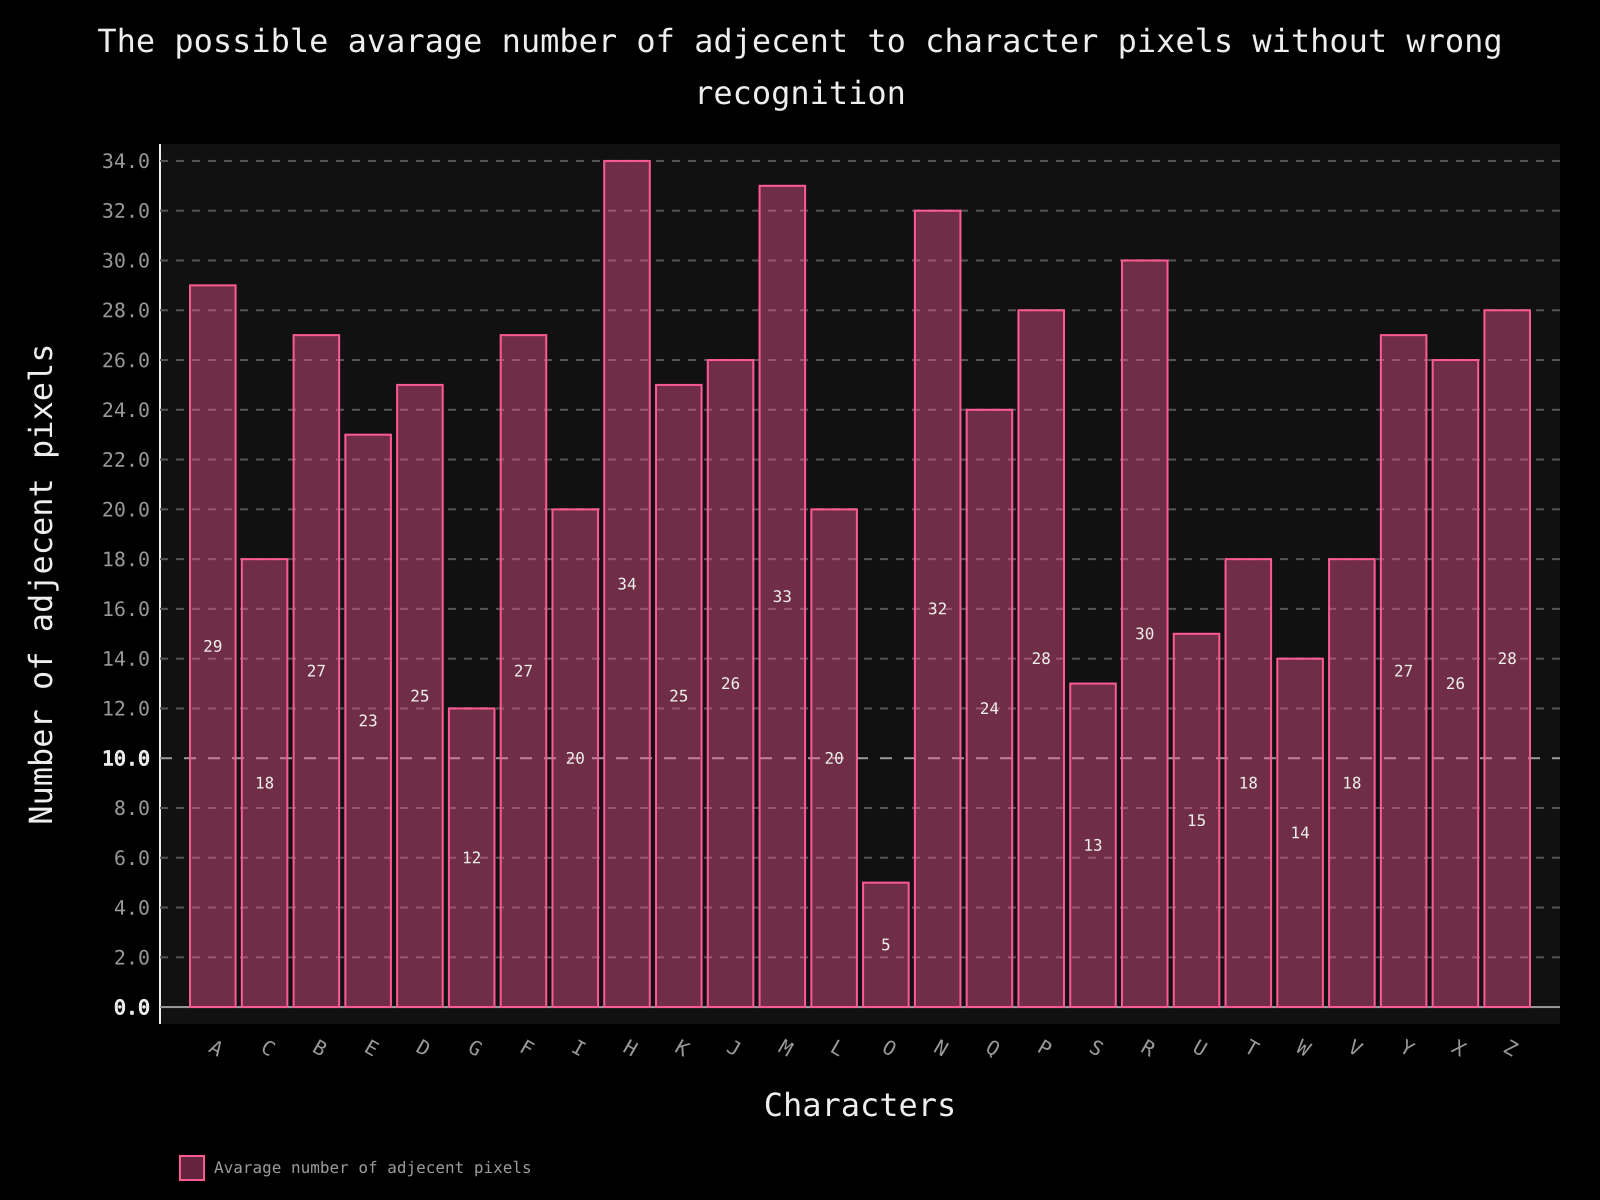
\includegraphics[scale=0.7,keepaspectratio=true]{Charts/AdjecentTestPlanResultsChart_ClasifierTester.png}	
	\caption{}
	\label{adjacent_clas}
\end{figure}

\clearpage
\subsection{Summarization of all tests}
All tests which were presented earlier in this paper were accumulated on one chart for both translation and classification.
Figures \ref{all_trans} and \ref{all_clas} show results of accumulated tests for classification and translation for all characters.
\begin{figure}[ht]
	\centering
	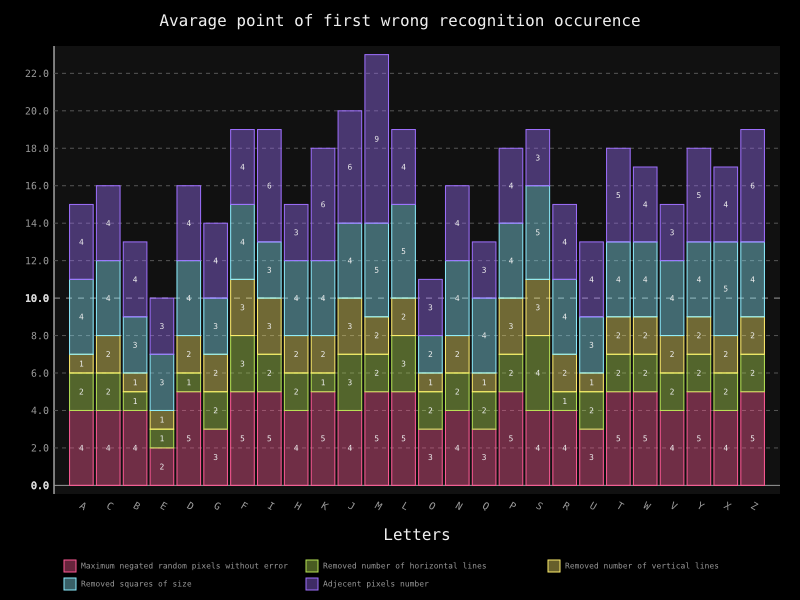
\includegraphics[scale=0.7,keepaspectratio=true]{Charts/AllTestPlanResultsChart_NormalTester.png}	
	\caption{}
	\label{all_trans}
\end{figure}

\begin{figure}[t]
	\centering
	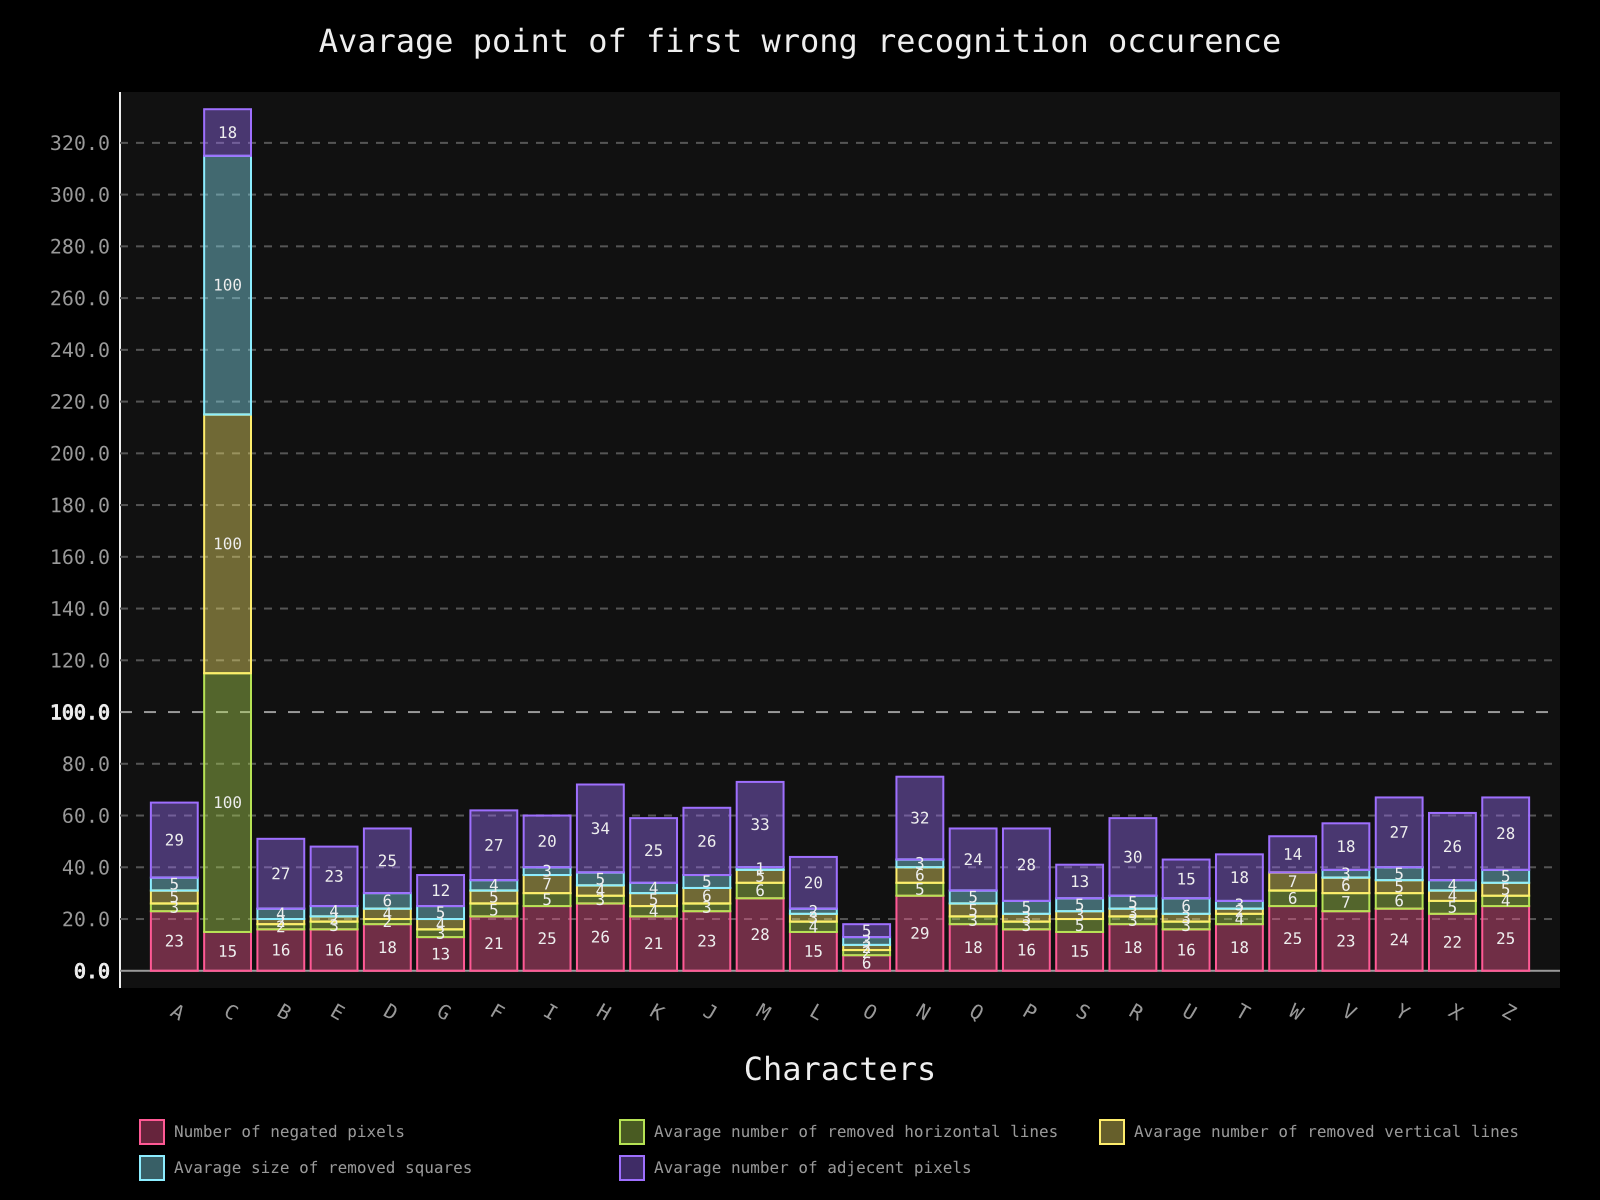
\includegraphics[scale=0.7,keepaspectratio=true]{Charts/AllTestPlanResultsChart_ClasifierTester.png}	
	\caption{}
	\label{all_clas}
\end{figure}
\clearpage
\pagebreak
\pagebreak
\section{Final remarks}
It can be noticed that some characters are easier to be recognized by engine.
On figure \ref{all_trans} and \ref{all_clas} it is visible that letters like O, U, G are much sensible for different distortions. In the other hand letters like K, M, H, with many lines are resistant to them.
Because it is much easier for network to give proper output for one class per one output neuron it is visible that automatic classification is much better than translation. There is no reson to use automatic translation because it gives much worse results trying to recognize characters with different noises and distortions.
Summarizing we have to admit that results exceeded our expectations. Correct recognition of letter with almost 30\% of additional pixels which make character more bold or 30\% of random noise is a really big number and could make hard to recognize character even for human.

\end{document}
